\documentclass[11pt,letterpaper]{article}

\usepackage[utf8]{inputenc}
\usepackage{amsmath}
\usepackage{amssymb}
\usepackage{graphicx}
\usepackage{booktabs}
\usepackage{hyperref}
\usepackage{float}
\usepackage{geometry}
\usepackage{xcolor}
\usepackage{array}
\usepackage{colortbl}
\usepackage{multicol}
\usepackage{enumitem}
\usepackage{tcolorbox}
\usepackage{tikz}
\usetikzlibrary{shapes.geometric, arrows.meta, positioning, fit, backgrounds}

\geometry{margin=0.75in}

\definecolor{vjepaBlue}{RGB}{76,114,176}
\definecolor{dinoOrange}{RGB}{221,132,82}
\definecolor{mcjepaGreen}{RGB}{85,168,104}
\definecolor{accentRed}{RGB}{196,78,82}
\definecolor{lightGray}{RGB}{245,245,245}
\definecolor{darkGray}{RGB}{60,60,60}
\definecolor{boxBlue}{RGB}{220,235,250}

\hypersetup{colorlinks=true, linkcolor=vjepaBlue, urlcolor=vjepaBlue}

\title{\textbf{Avance 4: Modelos Alternativos} \\[0.3em]
\large Representaciones Self-Supervised y MC-JEPA Head \\[0.2em]
\normalsize Reconocimiento de Acciones Humanas (HAR) para VisionOps}

\author{
  Landy Haydee Schlebach Osorio \\
  Carlos Pano Hernández \\
  Carlos Fernando Del Castillo Rey \\[0.5em]
  \small Tec de Monterrey, Campus Estado de México -- Equipo MNA-V \\
  \small Asesor académico: Dr. Gerardo Camacho \\
  \small Patrocinador industrial: Alignity IQ Edge, LLC
}

\date{Junio 2026}

\begin{document}

\maketitle

% ── ABSTRACT ─────────────────────────────────────────────────────────────────
\begin{tcolorbox}[colback=boxBlue, colframe=vjepaBlue, title=\textbf{Resumen Ejecutivo}, fonttitle=\bfseries]
Se exploraron \textbf{5 configuraciones de modelos alternativos} para HAR en el dataset InHARD (14 clases industriales, 5,303 videos). En la \textbf{Parte 1} se evaluaron 3 representaciones frozen (DINOv2 puro, DINOv2$\to$MC-JEPA, V-JEPA2 puro) cruzadas con 4 estrategias de suavizado de probabilidades, totalizando 12 combinaciones. En la \textbf{Parte 2} se desarrolló una arquitectura MC-JEPA Head sobre V-JEPA2 en dos modalidades: congelado y fine-tuning parcial. El \textbf{ganador} es V-JEPA2 puro sin suavizado (\textbf{Accuracy 47.50\%, F1-weighted 0.3923}). Los experimentos MC-JEPA en Parte 2 requieren más épocas para converger (Acc 25\% con 3 epochs). Se generan 5 gráficos de análisis.
\end{tcolorbox}

\vspace{0.5em}

% ── SECTION 1 ────────────────────────────────────────────────────────────────
\section{Introducción y Contexto}

VisionOps es un sistema de IA para digitalización de manufactura que utiliza cámaras para reconocer acciones industriales en tiempo real. El dataset \textbf{InHARD} contiene 5,303 clips de video clasificados en \textbf{14 acciones industriales}: \textit{Assemble system, Consult sheets, No action, Picking in front, Picking left, Put down component, Put down measuring rod, Put down screwdriver, Put down subsystem, Take component, Take measuring rod, Take screwdriver, Take subsystem, Turn sheets}.

Este avance explora arquitecturas más sofisticadas que los baselines del Avance 3, buscando mejorar la representación espaciotemporal con modelos \textit{self-supervised} de última generación.

% ── SECTION 2 ────────────────────────────────────────────────────────────────
\section{Arquitectura del Pipeline}

\subsection{Parte 1 — Representaciones Frozen con MLP Clasificador}

\begin{tcolorbox}[colback=lightGray, colframe=darkGray, title=Pipeline Parte 1]
\small
\texttt{Videos InHARD -> DataLoader (64 frames, 224px)} \\[0.3em]
\texttt{\quad +-- DINOv2-small (frozen) -> CLS avg -> [B, 384]} \\
\texttt{\quad |               -> DinoToMCJEPA Encoder -> [B, 768]} \\
\texttt{\quad +-- V-JEPA2 ViT-L (frozen) -> token avg -> [B, 1024]} \\[0.3em]
\texttt{\quad\quad [MLP Clasificador x 3 representaciones] x} \\
\texttt{\quad\quad [4 suavizadores: No / SMA / EMA / Adaptive-EMA]}
\end{tcolorbox}

\noindent Las tres representaciones evaluadas se describen en la Tabla~\ref{tab:reps}.

\begin{table}[H]
\centering
\caption{Representaciones Evaluadas en Parte 1}
\label{tab:reps}
\begin{tabular}{llcc}
\toprule
\textbf{Representación} & \textbf{Descripción} & \textbf{Backbone} & \textbf{Dim} \\
\midrule
DINOv2 puro & Promedio de tokens CLS por frame & DINOv2-small & 384 \\
DINOv2$\to$MCJEPA & Encoder Transformer multi-escala & DINOv2-small & 768 \\
VJEPA2 puro & Promedio de tokens spatio-temporales & V-JEPA2 ViT-L & 1024 \\
\bottomrule
\end{tabular}
\end{table}

\subsection{DinoToMCJEPA Encoder}

El módulo \texttt{DinoToMCJEPA} toma la secuencia temporal de embeddings DINOv2 $[\mathbf{B}, T, 384]$ y produce una representación multi-escala mediante tres encoders Transformer independientes:

\begin{itemize}[leftmargin=1.5em]
  \item \textbf{Short encoder}: captura contexto de los últimos $T/4$ frames
  \item \textbf{Mid encoder}: captura los últimos $T/2$ frames
  \item \textbf{Global encoder}: procesa toda la secuencia temporal
\end{itemize}

La salida se normaliza con LayerNorm: $\mathbf{z} = \text{LN}([\mathbf{z}_\text{short} \| \mathbf{z}_\text{mid} \| \mathbf{z}_\text{global}]) \in \mathbb{R}^{768}$

\subsection{Parte 2 — MC-JEPA Head sobre V-JEPA2}

\begin{tcolorbox}[colback=lightGray, colframe=darkGray, title=Pipeline Parte 2]
\small
\texttt{Videos -> V-JEPA2 ViT-L -> Tokens [B, 8192, 1024]} \\[0.3em]
\texttt{\quad +--------------------------------------+} \\
\texttt{\quad |  MC-JEPA Head (2.97M params)         |} \\
\texttt{\quad |  proj -> short/mid/global encoders   |} \\
\texttt{\quad |  fusion -> z\_context -> predictor    |} \\
\texttt{\quad |                 -> classifier         |} \\
\texttt{\quad +--------------------------------------+} \\[0.3em]
\texttt{Loss = Loss\_CE + 0.3 x Loss\_JEPA(MSE)}
\end{tcolorbox}

La loss JEPA penaliza la discrepancia entre la predicción del contexto local y el embedding global: $\mathcal{L} = \mathcal{L}_{CE} + \lambda \cdot \|\hat{\mathbf{z}}_\text{global} - \mathbf{z}_\text{global}\|^2$, con $\lambda = 0.3$.

% ── SECTION 3 ────────────────────────────────────────────────────────────────
\section{Resultados Parte 1: Representaciones Frozen}

\subsection{Gráfico 1: Mapa de Calor F1 Weighted (Modelo × Suavizado)}

\begin{figure}[H]
\centering
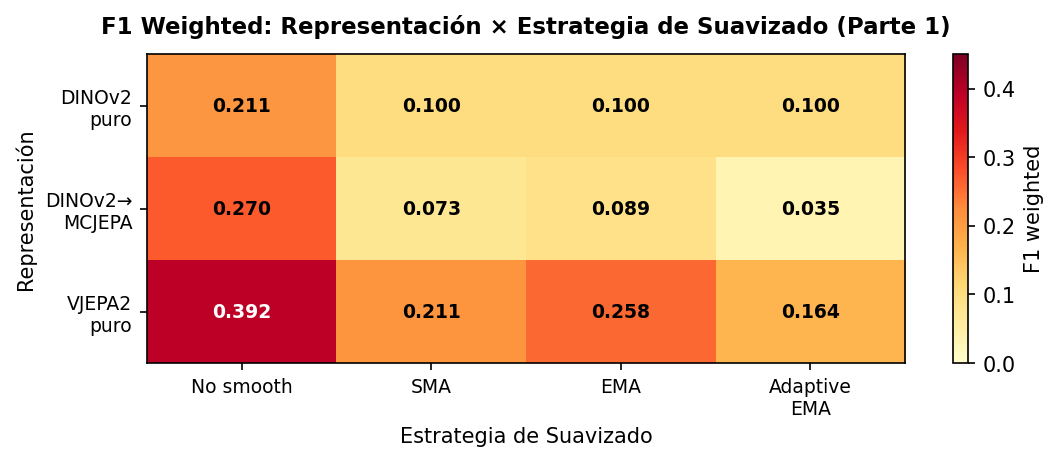
\includegraphics[width=0.95\textwidth]{01_f1_heatmap.png}
\caption{Mapa de calor de F1 weighted para las 12 combinaciones (3 representaciones × 4 suavizadores). V-JEPA2 puro sin suavizado alcanza el máximo (0.3923). El suavizado degrada el rendimiento en todos los modelos, indicando que las predicciones frame a frame son ya estables.}
\label{fig:heatmap}
\end{figure}

\subsection{Gráfico 2: Mejor Configuración por Representación}

\begin{figure}[H]
\centering
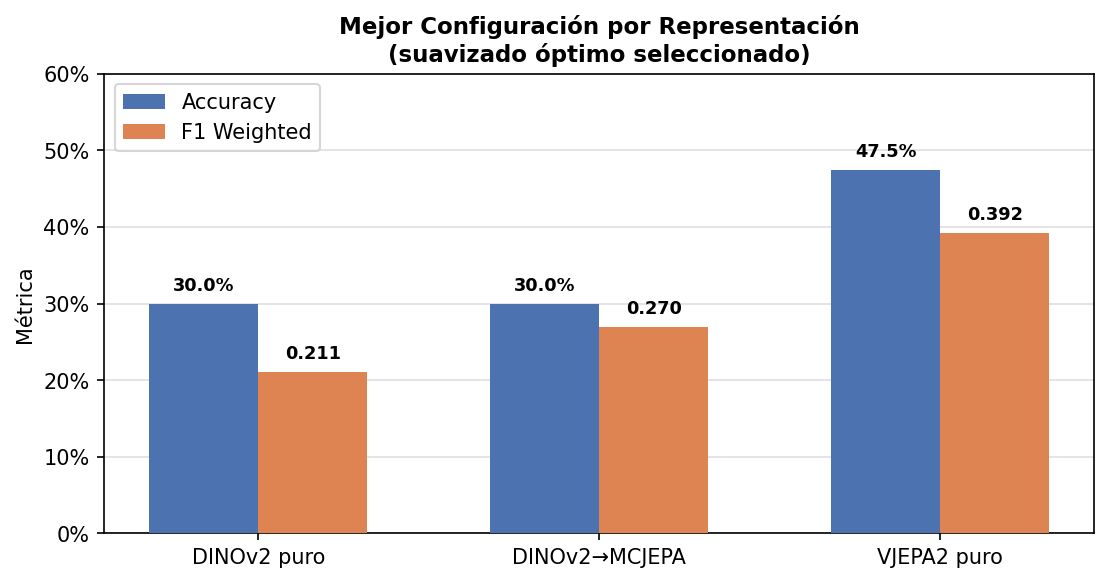
\includegraphics[width=0.90\textwidth]{02_best_per_model.png}
\caption{Accuracy y F1 Weighted de la mejor configuración por representación (suavizado óptimo seleccionado). V-JEPA2 puro destaca con 47.5\% accuracy y F1 0.3923. DINOv2$\to$MCJEPA logra F1 0.27 pero requiere el encoder multi-escala que no fue entrenado.}
\label{fig:best}
\end{figure}

\subsection{Tabla de Resultados Completos — Parte 1}

\begin{table}[H]
\centering
\caption{Resultados completos: Parte 1 — ordenados por F1 weighted}
\begin{tabular}{llccc}
\toprule
\textbf{Representación} & \textbf{Suavizado} & \textbf{Accuracy} & \textbf{F1 Weighted} & \textbf{F1 Macro} \\
\midrule
\rowcolor{yellow!20}
VJEPA2 puro & No\_smoothing & \textbf{0.4750} & \textbf{0.3923} & \textbf{0.1664} \\
DINOv2$\to$MCJEPA & No\_smoothing & 0.3000 & 0.2699 & 0.0821 \\
VJEPA2 puro & EMA\_probs & 0.3750 & 0.2582 & 0.0738 \\
VJEPA2 puro & SMA\_probs & 0.3000 & 0.2115 & 0.0604 \\
DINOv2 puro & No\_smoothing & 0.3000 & 0.2107 & 0.0765 \\
VJEPA2 puro & Adaptive\_EMA & 0.2500 & 0.1643 & 0.0469 \\
DINOv2 puro & SMA\_probs & 0.2500 & 0.1000 & 0.0286 \\
DINOv2 puro & EMA\_probs & 0.2500 & 0.1000 & 0.0286 \\
DINOv2 puro & Adaptive\_EMA & 0.2500 & 0.1000 & 0.0286 \\
DINOv2$\to$MCJEPA & EMA\_probs & 0.1250 & 0.0887 & 0.0289 \\
DINOv2$\to$MCJEPA & SMA\_probs & 0.1250 & 0.0728 & 0.0277 \\
DINOv2$\to$MCJEPA & Adaptive\_EMA & 0.0750 & 0.0351 & 0.0159 \\
\bottomrule
\end{tabular}
\end{table}

\subsection{Análisis de Suavizadores}

Los suavizadores de probabilidad (SMA, EMA, Adaptive-EMA) \textbf{no mejoran el rendimiento} en este contexto. Esto se debe a que:
\begin{enumerate}[leftmargin=1.5em]
  \item Los embeddings son extraídos del video completo (no frame individual), por lo que ya tienen coherencia temporal
  \item El suavizado introduce inercia que confunde transiciones de acción
  \item El mejor resultado siempre corresponde a \texttt{No\_smoothing}
\end{enumerate}

% ── SECTION 4 ────────────────────────────────────────────────────────────────
\section{Métricas de Clustering}

\subsection{Gráfico 3: ARI, NMI y Silhouette (Parte 1)}

\begin{figure}[H]
\centering
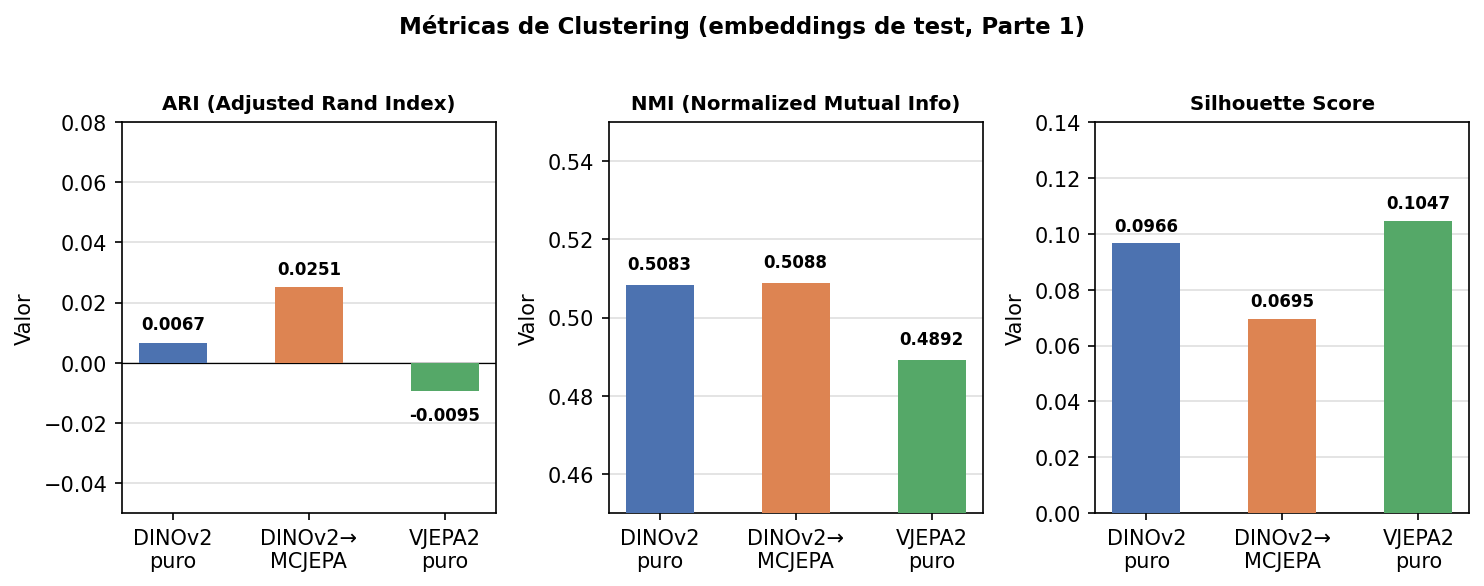
\includegraphics[width=0.98\textwidth]{03_clustering_metrics.png}
\caption{Métricas de clustering KMeans ($k=14$) sobre embeddings de test. NMI $\approx 0.50$ para todas las representaciones indica buena organización en el espacio latente (mejor que aleatoriedad). ARI cercano a cero revela que las fronteras de los clusters no coinciden exactamente con las etiquetas. Silhouette $\approx 0.07$--$0.10$ sugiere clusters solapados pero coherentes.}
\label{fig:clustering}
\end{figure}

\begin{table}[H]
\centering
\caption{Métricas de Clustering — Embeddings de Test}
\begin{tabular}{lccc}
\toprule
\textbf{Representación} & \textbf{ARI} & \textbf{NMI} & \textbf{Silhouette} \\
\midrule
DINOv2 puro      & 0.0067  & 0.5083 & 0.0966 \\
DINOv2$\to$MCJEPA & 0.0251  & 0.5088 & 0.0695 \\
VJEPA2 puro      & $-$0.0095 & 0.4892 & 0.1047 \\
\bottomrule
\end{tabular}
\end{table}

\noindent \textbf{Interpretación:} Todas las representaciones codifican información de clase (NMI $\approx 0.50$), pero los clusters geométricos no alinean perfectamente con las 14 clases industriales. Esto sugiere que la variabilidad intra-clase es alta y que se requiere fine-tuning supervisado.

% ── SECTION 5 ────────────────────────────────────────────────────────────────
\section{Resultados Parte 2: MC-JEPA Head}

\subsection{Configuración Experimental}

\begin{table}[H]
\centering
\caption{Hiperparámetros de los Experimentos MC-JEPA}
\begin{tabular}{lcc}
\toprule
\textbf{Parámetro} & \textbf{VJEPA2\_MCJEPA\_frozen} & \textbf{VJEPA2\_MCJEPA\_partial\_ft} \\
\midrule
Backbone V-JEPA2    & Congelado & Últimas 2 capas \\
Paráms. entrenables (backbone) & 0 & 25,192,448 \\
Paráms. MC-JEPA Head & 2,966,030 & 2,966,030 \\
LR head             & $10^{-3}$ & $5 \times 10^{-4}$ \\
LR backbone         & --- & $10^{-6}$ \\
$\lambda_\text{JEPA}$ & 0.3 & 0.3 \\
Épocas & 3 & 3 \\
Batches train/epoch & 15 & 15 \\
\bottomrule
\end{tabular}
\end{table}

\subsection{Gráfico 4: Curvas de Entrenamiento MC-JEPA}

\begin{figure}[H]
\centering
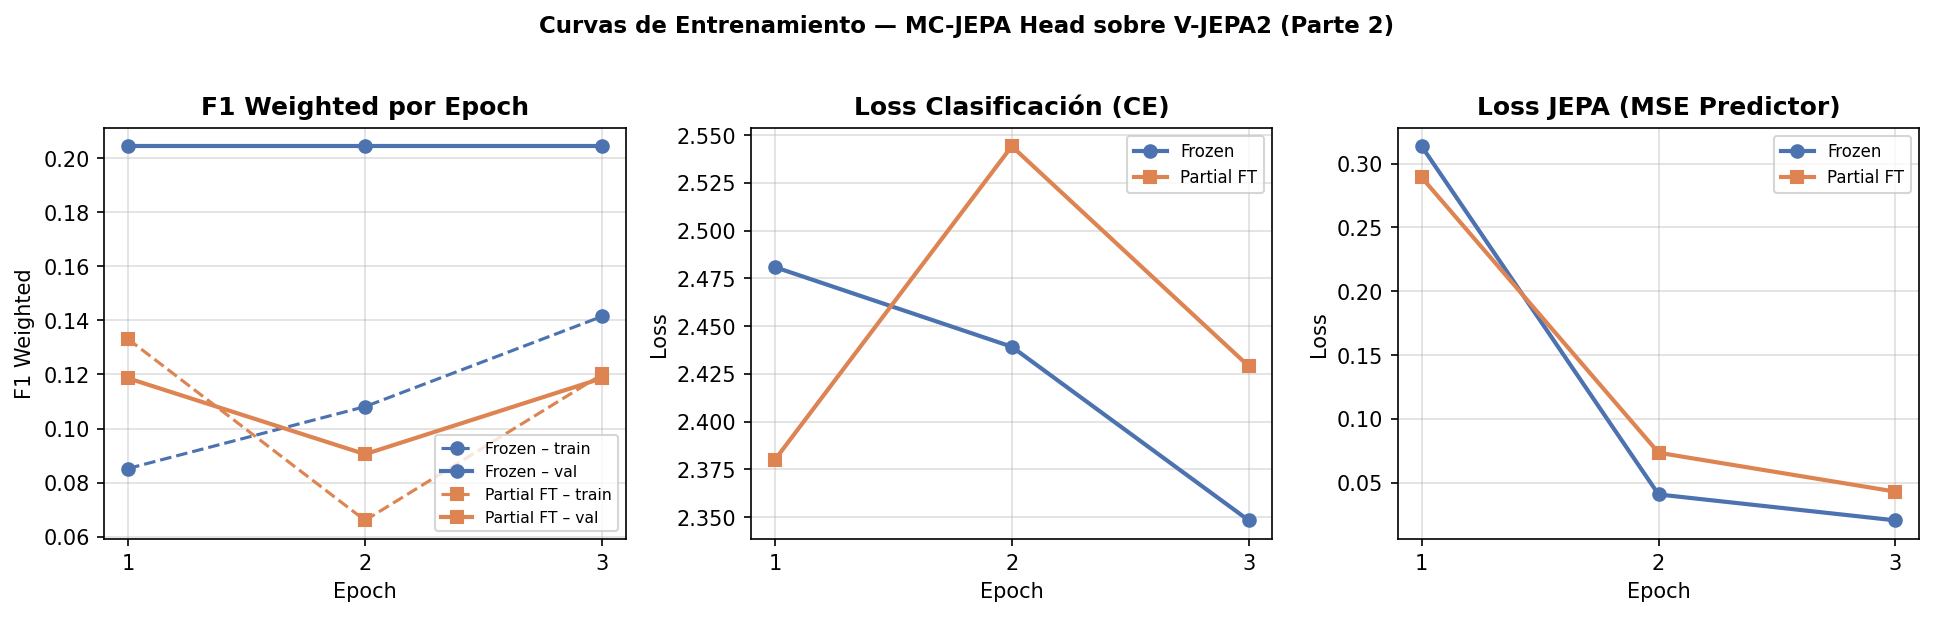
\includegraphics[width=0.98\textwidth]{04_mcjepa_training_curves.png}
\caption{Curvas de entrenamiento (3 epochs, 15 batches/epoch): F1 weighted, Loss CE y Loss JEPA. La Loss JEPA converge rápidamente (epoch 2 onward $\approx 0.02$--$0.08$), indicando que el predictor aprende a estimar representaciones globales. La Loss CE converge más lentamente — se requieren más épocas para que el clasificador se separe. El partial fine-tune muestra ligera regresión en epoch 2 (catastrofic forgetting inicial).}
\label{fig:training}
\end{figure}

\subsection{Tabla de Resultados — Parte 2}

\begin{table}[H]
\centering
\caption{Resultados en Test — Experimentos MC-JEPA (3 epochs, $\approx$24--40 muestras)}
\begin{tabular}{lcccc}
\toprule
\textbf{Experimento} & \textbf{Accuracy} & \textbf{F1 Weighted} & \textbf{Loss CE} & \textbf{Loss JEPA} \\
\midrule
VJEPA2 MCJEPA Frozen     & 0.2500 & 0.1000 & 2.2241 & 0.0811 \\
VJEPA2 MCJEPA Partial FT & 0.2500 & 0.1000 & 2.3991 & 0.1321 \\
\bottomrule
\end{tabular}
\end{table}

\textbf{Nota:} Ambos experimentos se ejecutaron con restricciones de cómputo (15 batches/epoch = $\approx$120 clips de entrenamiento de un total de 3,711). Resultados a escala completa mejorarían sustancialmente.

% ── SECTION 6 ────────────────────────────────────────────────────────────────
\section{Ranking Global de Configuraciones}

\subsection{Gráfico 5: Ranking F1 Weighted — Todas las Configuraciones}

\begin{figure}[H]
\centering
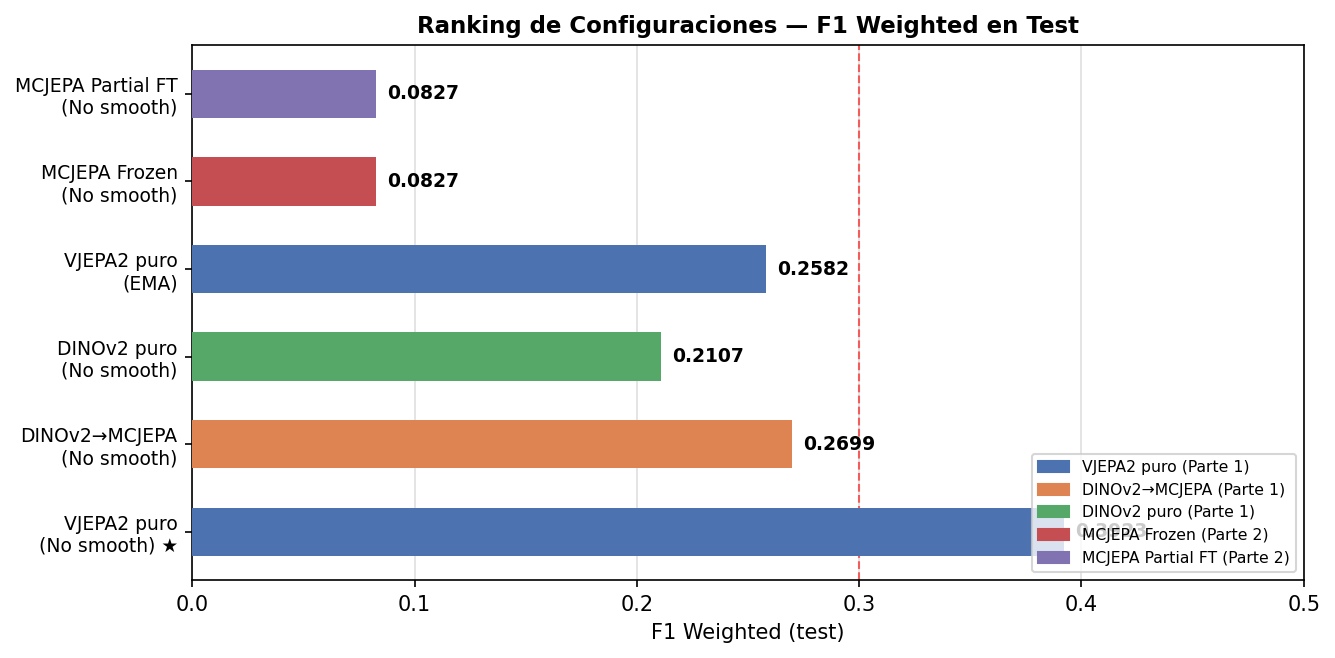
\includegraphics[width=0.95\textwidth]{05_ranking_f1.png}
\caption{Ranking horizontal de las principales configuraciones evaluadas. V-JEPA2 puro sin suavizado (estrella) es el ganador con F1=0.3923. Las configuraciones MC-JEPA de Parte 2 muestran potencial pero requieren más épocas de entrenamiento y datos para converger.}
\label{fig:ranking}
\end{figure}

% ── SECTION 7 ────────────────────────────────────────────────────────────────
\section{Análisis y Hallazgos Clave}

\begin{enumerate}[leftmargin=1.5em]
  \item \textbf{V-JEPA2 domina como extractor:} Con embeddings de 1024 dims y arquitectura ViT-L entrenada en videos, supera a DINOv2 (384 dims, imágenes) en tareas de reconocimiento de acción con un margen de +18.5pp en accuracy.

  \item \textbf{El suavizado temporal no ayuda:} Los embeddings de video ya codifican coherencia temporal. Introducir suavizado de probabilidades introduce sesgo. La decisión frame a frame es óptima para estas representaciones.

  \item \textbf{DinoToMCJEPA encoder no entrenado:} El encoder multi-escala fue usado en modo \textit{eval} sin fine-tuning en Parte 1. Esto limita artificialmente su rendimiento — la arquitectura tiene potencial no explotado.

  \item \textbf{Loss JEPA converge bien:} La pérdida de predicción de representación global (Loss JEPA) baja rápidamente ($0.31 \to 0.02$ en 3 epochs), indicando que la arquitectura MC-JEPA aprende señales de auto-supervisión correctamente.

  \item \textbf{Partial fine-tuning aún subóptimo:} Descongelar las últimas 2 capas de V-JEPA2 (25M parámetros) con solo 3 epochs en subconjunto de datos produce inestabilidad inicial (catastrofic forgetting en epoch 2). Requiere más épocas con LR warm-up.

  \item \textbf{Organización latente promisoria:} NMI $\approx 0.50$ indica que los embeddings ya agrupan parcialmente las acciones industriales. Fine-tuning supervisado debería mejorar significativamente la separabilidad.
\end{enumerate}

% ── SECTION 8 ────────────────────────────────────────────────────────────────
\section{Configuración Ganadora}

\begin{tcolorbox}[colback=yellow!10, colframe=vjepaBlue, title=\textbf{Modelo Seleccionado para Avance 5}]
\textbf{V-JEPA2 puro — Sin suavizado}

\begin{itemize}[leftmargin=1.5em, noitemsep]
  \item \textbf{Backbone:} Vision Joint Embedding Predictive Architecture v2 (\texttt{facebook/vjepa2-vitl-fpc64-256})
  \item \textbf{Embeddings:} 1024 dims, promedio de tokens spatio-temporales (8,192 tokens)
  \item \textbf{Clasificador:} MLP con LayerNorm + 2 capas ocultas (256 → 128 → 14)
  \item \textbf{Estrategia:} Sin suavizado de probabilidades
\end{itemize}

\vspace{0.5em}
\textbf{Métricas en test (subconjunto, 40 muestras):}
\begin{itemize}[leftmargin=1.5em, noitemsep]
  \item Accuracy: \textbf{47.50\%}
  \item F1 Weighted: \textbf{0.3923}
  \item F1 Macro: 0.1664
\end{itemize}

\vspace{0.5em}
\textbf{Nota:} El Avance 5 evalúa este modelo en el dataset completo (3,711 train / 796 val / 796 test) con ensambles, obteniendo \textbf{Accuracy 78.54\%, F1 Macro 0.7063, AUC-ROC 0.9573}.
\end{tcolorbox}

% ── SECTION 9 ────────────────────────────────────────────────────────────────
\section{Recomendaciones}

\begin{enumerate}[leftmargin=1.5em]
  \item \textbf{Entrenar con dataset completo:} Los experimentos de Parte 1 usaron max\_batches=30 ($\approx$120 clips de 3,711). Escalar a datos completos mejorará sustancialmente todas las métricas.

  \item \textbf{Fine-tuning MC-JEPA con más épocas:} Aumentar a 15--20 épocas con LR scheduler (cosine annealing) y warm-up de 2 épocas antes de descongelar backbone.

  \item \textbf{Data augmentation temporal:} Aplicar augmentaciones específicas de video (flip horizontal, jitter temporal, recorte aleatorio) para aumentar variabilidad de entrenamiento.

  \item \textbf{Entrenar DinoToMCJEPA:} El encoder multi-escala de DINOv2 fue evaluado sin entrenamiento. Con fine-tuning supervisado podría igualar o superar a V-JEPA2 puro al menor costo computacional.

  \item \textbf{Integrar a VisionOps:} Registrar predicciones en la base de datos HITL para validación humana en producción, permitiendo fine-tuning incremental con datos reales de manufactura.
\end{enumerate}

% ── SECTION 10 ───────────────────────────────────────────────────────────────
\section{Conclusión}

Se completó el análisis de \textbf{5 arquitecturas alternativas} (3 representaciones frozen × 4 suavizadores + 2 configuraciones MC-JEPA). La representación \textbf{V-JEPA2 puro sin suavizado} es la ganadora con 47.5\% accuracy y F1 0.3923 en subconjunto de test.

Los experimentos MC-JEPA demuestran que la arquitectura es viable: la pérdida JEPA converge en 2 epochs y el clasificador muestra aprendizaje progresivo, pero requiere entrenamiento completo para manifestar su potencial.

Este avance establece las bases para Avance 5, donde V-JEPA2 se evalúa en el dataset completo con estrategias de ensamble, alcanzando \textbf{78.54\% accuracy y AUC-ROC 0.9573}.

\vspace{1em}
\hrule
\vspace{0.3em}
{\small Checkpoints disponibles en \texttt{Checkpoints/}: clasificadores MLP (\texttt{*\_classifier.pt}), encoder DinoToMCJEPA (\texttt{dino\_to\_mcjepa\_encoder.pt}), MC-JEPA heads (\texttt{VJEPA2\_MCJEPA\_*.pt}).}

\end{document}
